\documentclass[12pt,english]{article}
\usepackage[a4paper,bindingoffset=0.2in,%
            left=1in,right=1in,top=1in,bottom=1in,%
            footskip=.25in]{geometry}
\usepackage{blindtext}
\usepackage{titling}
\usepackage{amssymb}
\usepackage{amsmath}
\usepackage{listings}
\usepackage{lettrine} 
\usepackage{tikz}  
\usepackage{color} 
\usepackage{verbatim}
 \usetikzlibrary{shapes, arrows, calc, arrows.meta, fit, positioning} % these are the parameters passed to the library to create the node graphs  
\tikzset{  
    -Latex,auto,node distance =0.6 cm and 1.3 cm, thick,% node distance is the distance between one node to other, where 1.5cm is the length of the edge between the nodes  
    state/.style ={ellipse, draw, minimum width = 0.9 cm}, % the minimum width is the width of the ellipse, which is the size of the shape of vertex in the node graph  
    point/.style = {circle, draw, inner sep=0.18cm, fill, node contents={}},  
    bidirected/.style={Latex-Latex,dashed}, % it is the edge having two directions  
    el/.style = {inner sep=2.5pt, align=right, sloped}  
}  
\tikzset{
  treenode/.style = {shape=rectangle, rounded corners,
                     draw, align=center,
                     top color=white, bottom color=blue!20},
  root/.style     = {treenode, font=\Large, bottom color=red!30},
  env/.style      = {treenode, font=\ttfamily\normalsize},
  dummy/.style    = {circle,draw}
}
\setlength{\parskip}{12pt}
\title{Home Work 1 Undergraduate}
\date{\today}
\author{Jose Carlos Munoz}
%================================
\begin{document}
\newgeometry{left=0.8in,right=0.8in,top=1in,bottom=1in}
\begin{center}
    \Large
    \textbf{Homework 2}\\
    \small
    \today\\
    \large
    Jose Carlos Munoz
\end{center}%===============================
3.2c)\\
\begin{equation}\tag{1}\label{eq:1}
\begin{split}
Gini_{Male} &= 1- (\frac{4}{10})^{2} - (\frac{6}{10})^{2}\\
&=0.48
\end{split}
\end{equation}
%===============================
\begin{equation}\tag{2}\label{eq:2}
\begin{split}
Gini_{Female} &= 1- (\frac{4}{10})^{2} - (\frac{6}{10})^{2}\\
&=0.48
\end{split}
\end{equation}
%===============================
\begin{equation}\tag{3}\label{eq:3}
\begin{split}
Gini_{Gender} &= \frac{10}{20}*Gini_{Male} + \frac{10}{20}*Gini_{Female}\\
&=0.48
\end{split}
\end{equation}
%===============================
The Gini for Male is as showin in\eqref{eq:1}\\
The Gini for Female is as showin in\eqref{eq:2}\\
The Gini for gender is as showin in\eqref{eq:3}\\ \\
%===============================
%===============================
3.2d)\\
\begin{equation}\tag{1}\label{eq:4}
\begin{split}
Gini_{Family} &= 1- (\frac{1}{4})^{2} - (\frac{3}{4})^{2}\\
&=0.375
\end{split}
\end{equation}
%===============================
\begin{equation}\tag{2}\label{eq:5}
\begin{split}
Gini_{Sports} &= 1- (\frac{8}{8})^{2} - (\frac{0}{8})^{2}\\
&=0.00
\end{split}
\end{equation}
%===============================
\begin{equation}\tag{3}\label{eq:6}
\begin{split}
Gini_{Luxury} &= 1- (\frac{1}{8})^{2} - (\frac{7}{8})^{2}\\
&=0.21875
\end{split}
\end{equation}
%===============================
\begin{equation}\tag{4}\label{eq:7}
\begin{split}
Gini_{Cars} &= \frac{4}{20}*Gini_{Family} + \frac{8}{20}*Gini_{Sports}+ \frac{8}{20}*Gini_{Luxury}\\
&=0.1625
\end{split}
\end{equation}
The Gini for Family is as showin in\eqref{eq:5}\\
The Gini for Sports is as showin in\eqref{eq:6}\\
The Gini for Luxury is as showin in\eqref{eq:7}\\
The Gini for Cars is as showin in\eqref{eq:8}\\ \\
%===============================
%===============================
3.2e)\\
\begin{equation}\tag{1}\label{eq:9}
\begin{split}
Gini_{Small} &= 1- (\frac{2}{5})^{2} - (\frac{3}{5})^{2}\\
&=.48
\end{split}
\end{equation}
%===============================
\begin{equation}\tag{2}\label{eq:10}
\begin{split}
Gini_{Medium} &= 1- (\frac{3}{7})^{2} - (\frac{4}{7})^{2}\\
&=\frac{24}{49}
\end{split}
\end{equation}
%===============================
\begin{equation}\tag{3}\label{eq:11}
\begin{split}
Gini_{Large} &= 1- (\frac{3}{4})^{2} - (\frac{1}{4})^{2}\\
&=0.5
\end{split}
\end{equation}
%===============================
\begin{equation}\tag{4}\label{eq:12}
\begin{split}
Gini_{Extra_Large} &= 1- (\frac{2}{4})^{2} - (\frac{2}{4})^{2}\\
&=0.5
\end{split}
\end{equation}
%===============================
\begin{equation}\tag{5}\label{eq:13}
\begin{split}
Gini_{Shirt_Size} &= \frac{5}{20}*Gini_{Small} + \frac{7}{20}*Gini_{Medium} + \frac{4}{20}*Gini_{Large} + \frac{4}{20}*Gini_{Extra_Large}\\
&=0.4914
\end{split}
\end{equation}
The Gini for Small is as showin in\eqref{eq:9}\\
The Gini for Medium is as showin in\eqref{eq:10}\\
The Gini for Large is as showin in\eqref{eq:11}\\
The Gini for Extra Large is as showin in\eqref{eq:12}\\
The Gini for Shirt Size is as showin in\eqref{eq:13}\\ \\
%===============================
%===============================
3.2f)\\
The Car type because it has the lowest Gini Index.\\\\
%===============================
%===============================
3.5a)\\
\begin{equation}\tag{1}\label{eq:14}
\begin{split}
E_{orig} &= - \frac{4}{10} *log(\frac{4}{10}) - \frac{6}{10} *log(\frac{6}{10})\\
&=.9710
\end{split}
\end{equation}
%===============================
The  overall Entropy before the split is shown in \eqref{eq:14}\\
\begin{equation}\tag{2}\label{eq:15}
\begin{split}
E_{T} &= - \frac{4}{7} *log(\frac{4}{7}) - \frac{3}{7} *log(\frac{4}{7})\\
E_{F} &= - \frac{3}{3} *log(\frac{3}{3}) - \frac{0}{3} *log(\frac{0}{0})\\
\Delta E &=E{orig} - \frac{7}{10} * E_{T} - \frac{3}{10} * E_{F}\\
 &=0.2813
\end{split}
\end{equation}
%===============================
The data gain from the splitting for A is show in \eqref{eq:15}\\
\begin{equation}\tag{3}\label{eq:16}
\begin{split}
E_{T} &= - \frac{3}{4} *log(\frac{3}{4}) - \frac{1}{4} *log(\frac{1}{4})\\
E_{F} &= - \frac{1}{6} *log(\frac{1}{6}) - \frac{5}{6} *log(\frac{5}{6})\\
\Delta E &=E{orig} - \frac{4}{10} * E_{T} - \frac{6}{10} * E_{F}\\
 &=0.2565
\end{split}
\end{equation}
%===============================
The data gain from the splitting for B is show in \eqref{eq:16}\\ \\
3.7a)\\
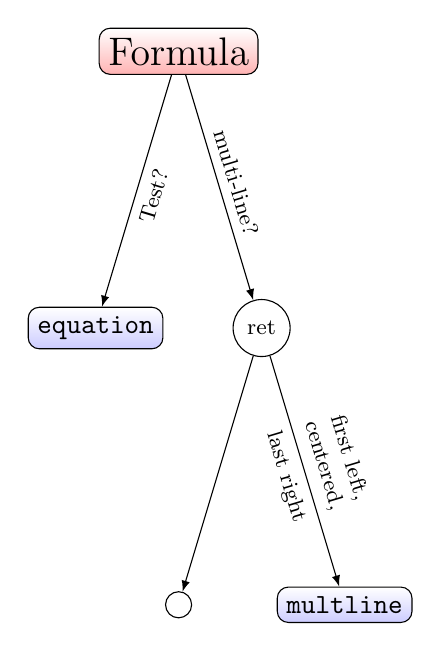
\begin{tikzpicture}
  [
    grow                    = down,
    sibling distance        = 6em,
    level distance          = 10em,
    edge from parent/.style = {draw, -latex},
    every node/.style       = {font=\footnotesize},
    sloped
  ]
  \node [root] {Formula}
    child { node [env] {equation}
      edge from parent node [below] {Test?} }
    child { node [dummy] {ret}
      child { node [dummy] {}}
      child { node [env] {multline}
              edge from parent node [above, align=center]
                {first left,\\centered,}
              node [below] {last right}}
              edge from parent node [above] {multi-line?} };
\end{tikzpicture}
\\
%===============================
%===============================
3.7b)\\
answer 1
3.7c)\\
answer 1\\
3.7a)\\
answer 1\\
3.7b)\\
answer 1
3.7c)\\
\end{document}
